\documentclass{handout}

% \SetInstructor{ Lt Col James Phillips}
\SetCourseTitle{ECE231: Electrical Circuits and Systems I}
\SetSemester{Fall 2016}
\SetHandoutTitle{Lecture 6: Node Voltage Analysis}
%\SetDueDate{1 Jan 2016}
%\ShowAllBlanks
\usepackage{listings}
\showsoln \setsolncolor{red}

\begin{document}
\maketitle


\textbf{OBJECTIVES:}
\begin{enumerate}
\item Demonstrate the ability to write node voltage equations for a given circuit
\item Demonstrate the ability to solve for unknown circuit parameters using node voltage analysis
\end{enumerate}

\textbf{READING}
\begin{description}
\item [Required]:
\begin{itemize}
\item  Textbook, section 3.1, pages 73-91
\end{itemize}
\item [Optional]: None
\end{description}


\section{What is Node Voltage Analysis?}
Relying on element constraints (e.g., component i-v relationships) and connection constraints (e.g., KVL and KCL) to solve complex circuits can lead to unwieldy numbers of equations.  Instead we can write equations for {\em Node Voltages}.  This is referred to as node voltage analysis.  We start by learning the steps for writing node voltage equations and then looking at methods to solve those equations.

\newpage
\pagebreak
\clearpage

\section{Circuits with NO VOLTAGE source}
Without justification I will offer that node voltage analysis is easier when no voltage sources are in the circuit.  These circuits contain only current sources and resistors.  We will start by looking at these types of circuits.

\subsection{How do we write Node Voltage equations?}
Below are the steps for writing node voltage equations:
\soln{4in}{
\begin{enumerate}
\item Identify a \textbf{reference node}.  You will not write an equation for this node, but the voltages at the other nodes will use this as a reference.
\item Write \textbf{KCL equations} at the other $N-1$ nodes
\item Write the currents in the KCL equations in terms of \textbf{node voltages} and resistances
\item Rearrange the equations above into \textbf{standard form}
\end{enumerate}
}
\newpage
\pagebreak
\clearpage

\subsection{Examples}
\textbf{Textbook Exercise 3--4} Formulate node voltage equations for the circuit in Figure \ref{fig: NodalAnalysisEx1} and place the results in matrix form ($\mathbf{Ax}=\mathbf{b}$)
\begin{figure} [h t b]
\centering
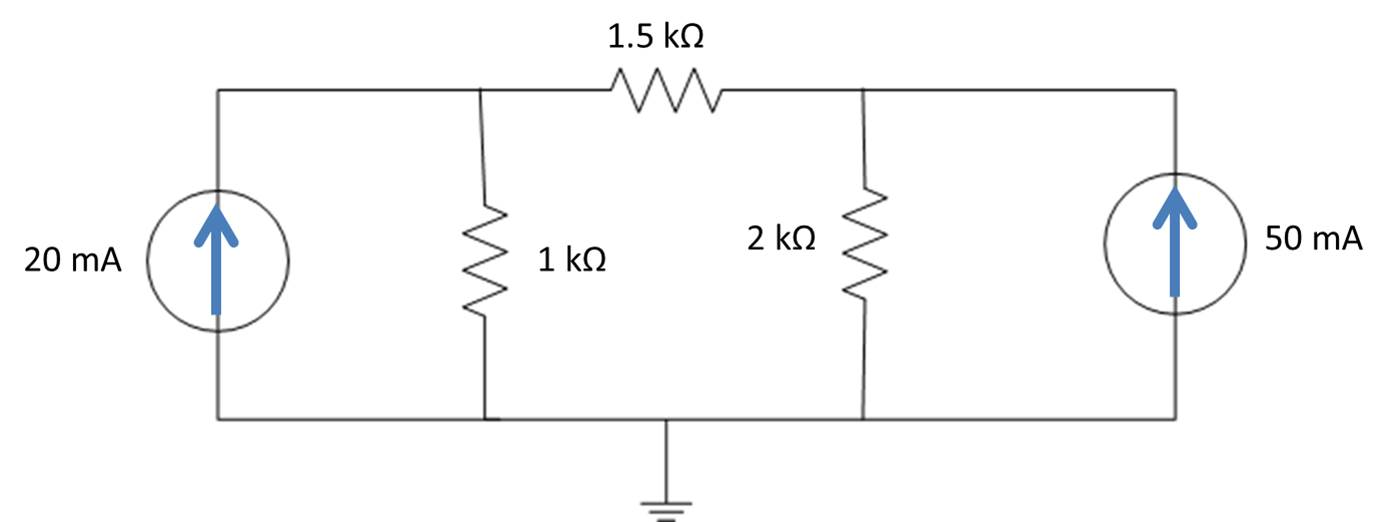
\includegraphics[width=0.7\textwidth]{NodalAnalysisEx1.jpg}
\caption{Circuit for textbook exercise 3--4}
\label{fig: NodalAnalysisEx1}
\end{figure}
\soln{6in}{
\begin{figure} [h t b]
\centering
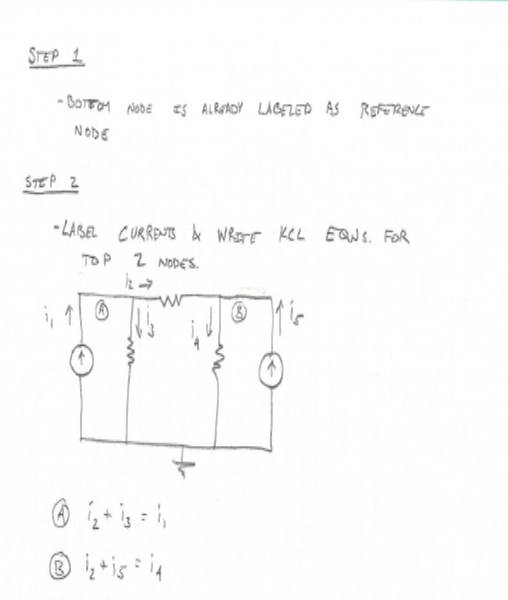
\includegraphics[width=0.8\textwidth]{NodalAnalysisEx1solnA.jpg}
\end{figure}

\begin{figure} [h t b]
\centering
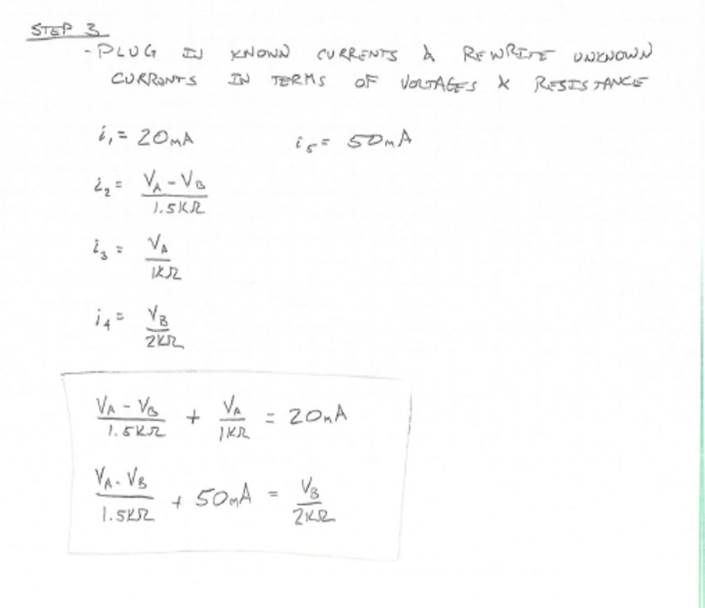
\includegraphics[width=0.8\textwidth]{NodalAnalysisEx1solnB.jpg}
\end{figure}

\begin{figure} [h t b]
\centering
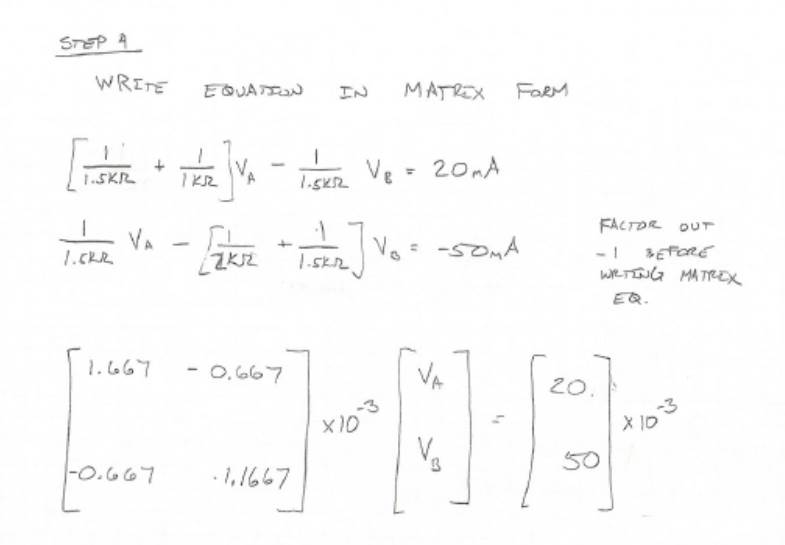
\includegraphics[width=0.8\textwidth]{NodalAnalysisEx1solnC.jpg}
\end{figure}
}

\newpage
\pagebreak
\clearpage

\textbf{Example 2} -- Use Node Voltage Analysis to solve for all node voltages in Figure \ref{fig: NodalAnalysisEx2}
\begin{figure} [h t b]
\centering
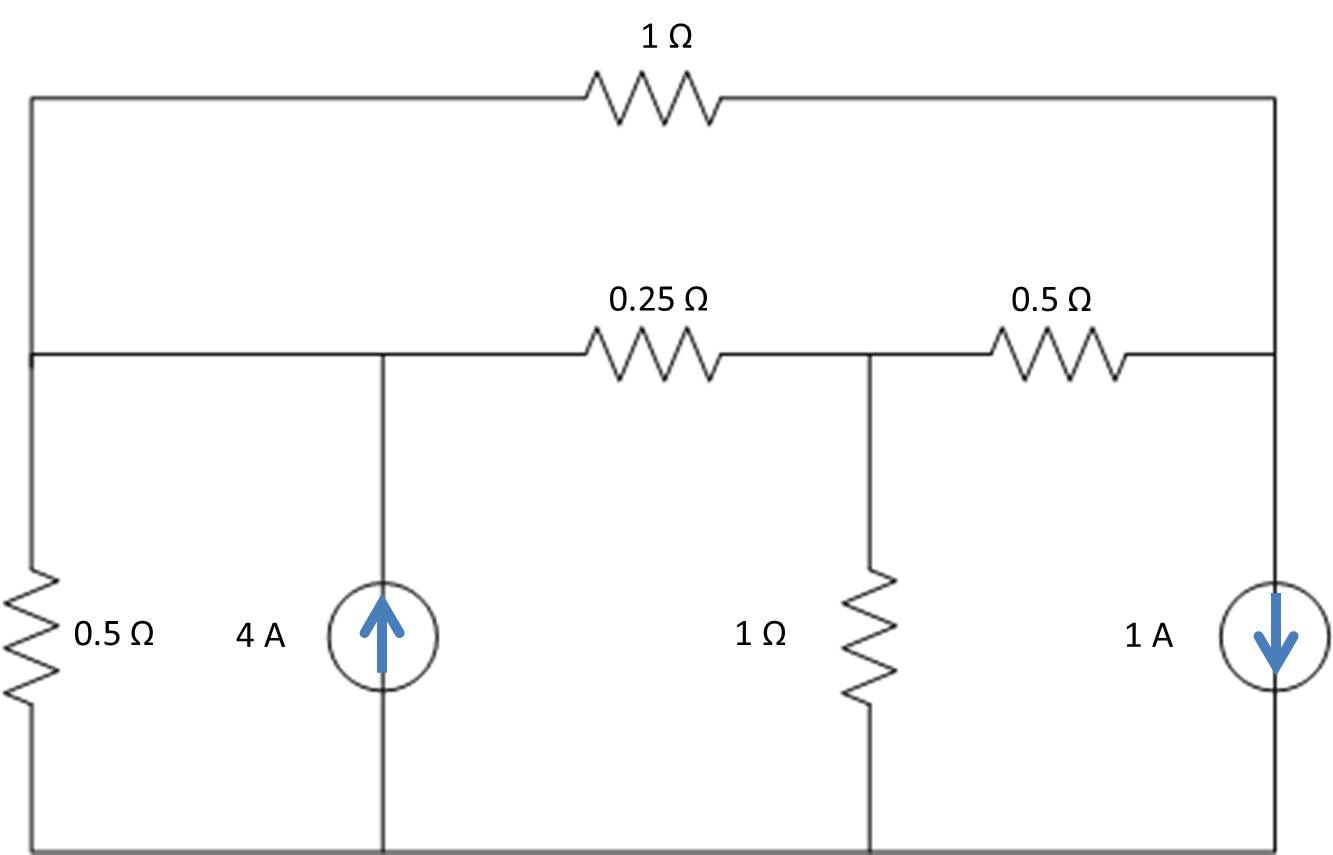
\includegraphics[width=0.7\textwidth]{NodalAnalysisEx2.jpg}
\caption{Circuit for Example 2}
\label{fig: NodalAnalysisEx2}
\end{figure}
\soln{6in}{
\begin{figure} [h t b]
\centering
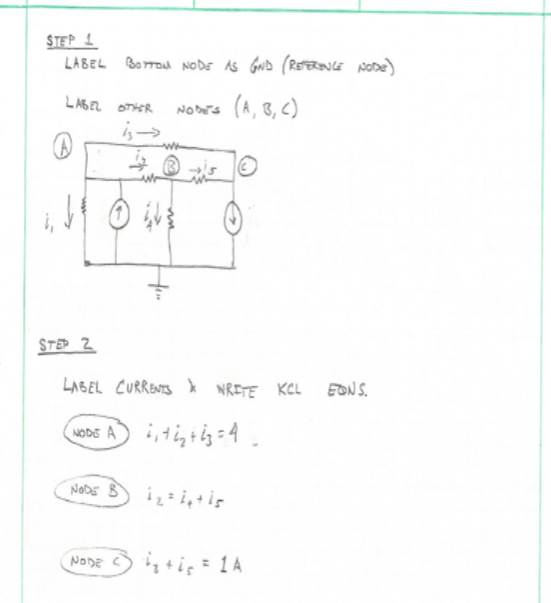
\includegraphics[width=0.7\textwidth]{NodalAnalysisEx2solnA.jpg}
\end{figure}

\begin{figure} [h t b]
\centering
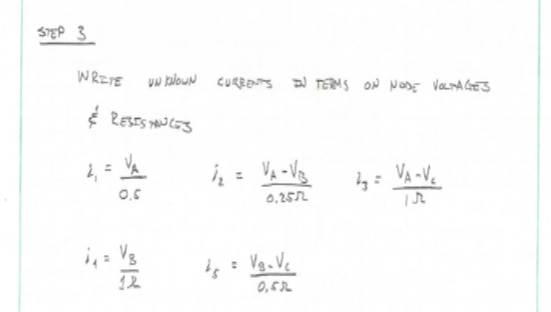
\includegraphics[width=0.7\textwidth]{NodalAnalysisEx2solnB.jpg}
\end{figure}

\begin{figure} [h t b]
\centering
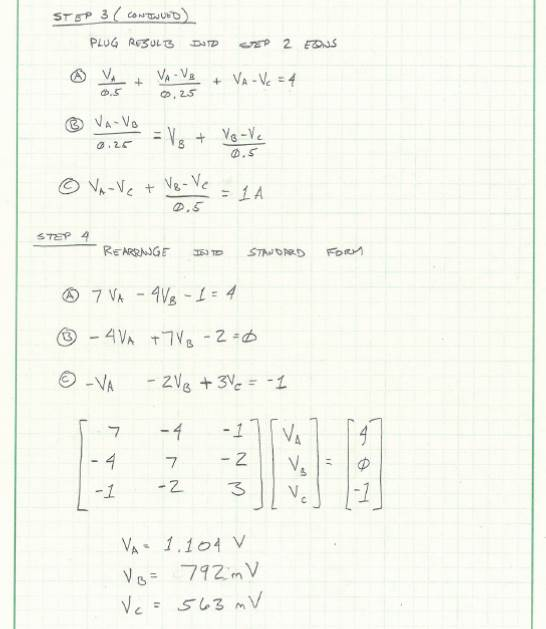
\includegraphics[width=0.7\textwidth]{NodalAnalysisEx2solnC.jpg}
\end{figure}
}

\newpage
\pagebreak
\clearpage

\section{Node Voltage Analysis WITH Voltage Sources}
When you have a voltage source in a circuit it will complicate Node Voltage Analysis slightly.  This is because the first step in the process is to apply KCL at the nodes, but we cannot directly know the current into or out of an ideal voltage source. While it complicates the first step of the process, over all it will make most problems easier by reducing the number of node equations.

We will look at 3 different methods that can be used to solve these problems.  You will need to  understand all three, since they apply in different circumstances. Complex circuits may require you employ 2 or even all 3 of these methods.

\subsection{Method 1: Source Transformation}
If your voltage source is in series with a resistor, you should do a source transformation to get rid of your voltage source.  You then revert back to the 4--step process for circuits without voltage sources. Figure \ref{fig: SourceTransformation} shows a reminder on how to transform voltage sources.
\begin{figure} [h t b]
\centering
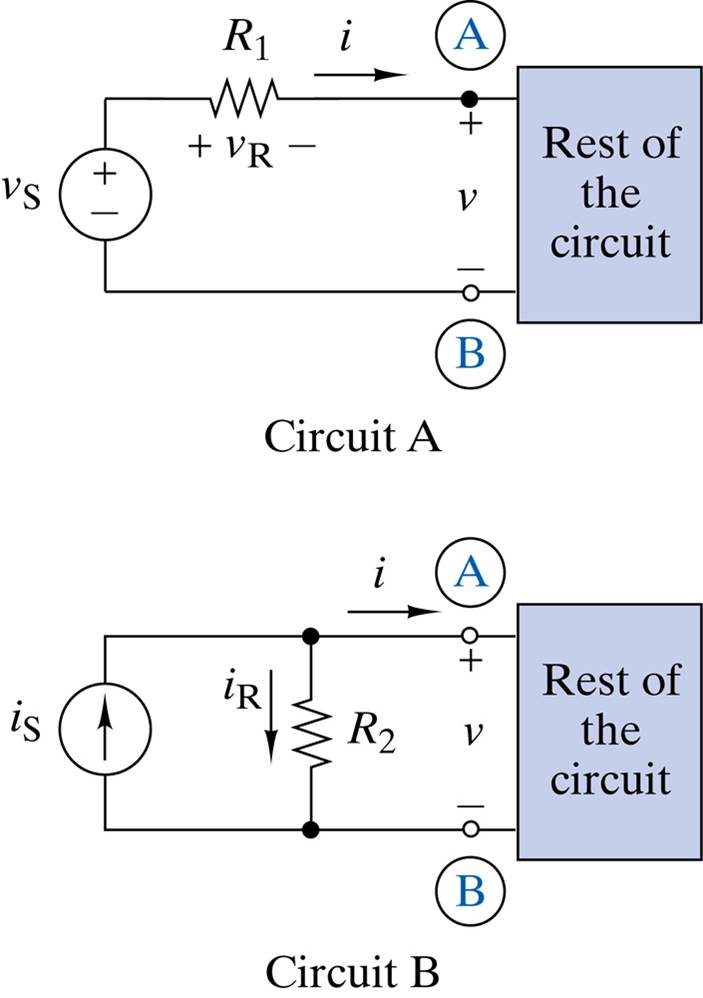
\includegraphics[width=0.4\textwidth]{SourceTransformation.jpg}
\caption{A quick reminder on source transformation}
\label{fig: SourceTransformation}
\end{figure}

where $i$ and $v$ are related by
\begin{eqnarray}
v_s &=& i_sR_2 \nonumber \\
i_s &=& \frac{v_s}{R_1} \nonumber \\
R_1 &=& R_2 \nonumber
\end{eqnarray}
\newpage
\pagebreak
\clearpage

\textbf{Textbook Exercise 3-9}: In Figure \ref{fig: TextbookExercise3-9}, use source transformation and Node Voltage Analysis to find the voltage across the $10k\ \Omega$ resistor.
\begin{figure} [h t b]
\centering
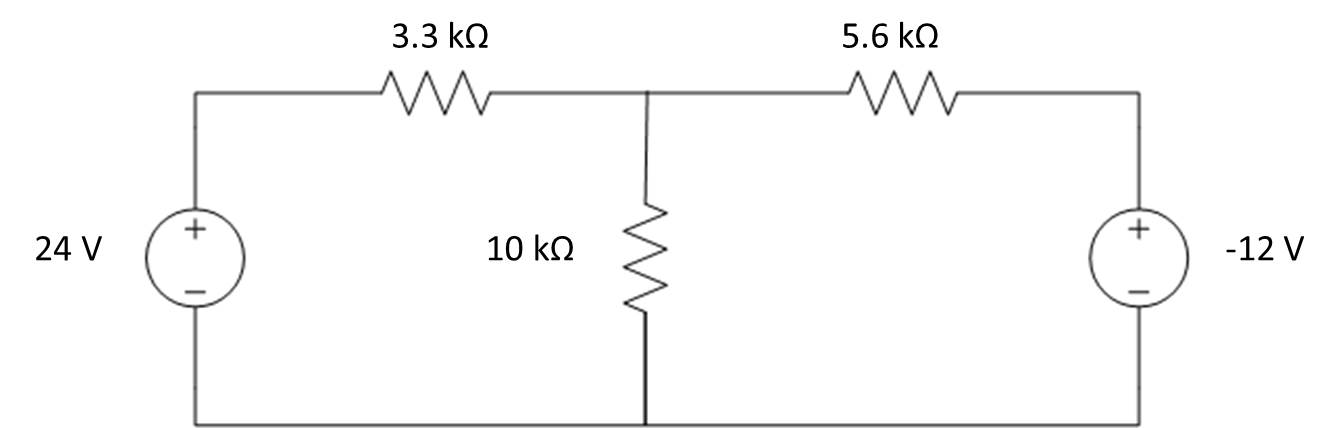
\includegraphics[width=0.5\textwidth]{TextbookExercise3-9.jpg}
\caption{Circuit for Textbook Exercise 3-9}
\label{fig: TextbookExercise3-9}
\end{figure}
\soln{4in}{
\begin{figure} [h t b]
\centering
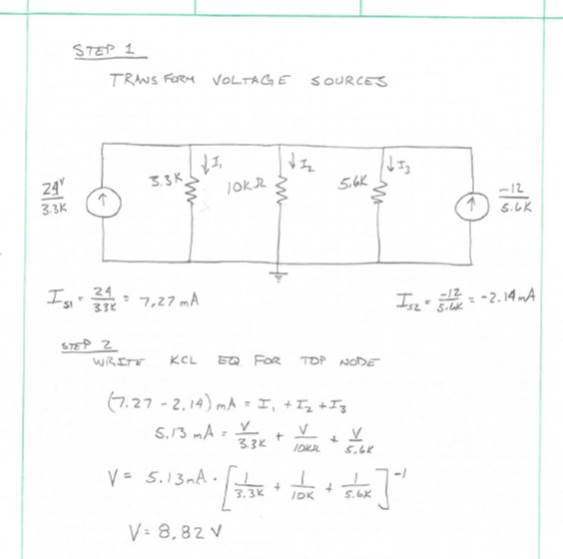
\includegraphics[width=0.8\textwidth]{TextbookExercise3-9solnM1.jpg}
\end{figure}
}


\newpage
\pagebreak
\clearpage

\subsection{Method 2: Smart choice of reference node}
You should always think about what node makes the most sense as a reference node.  When possible select one of the nodes that connects to your voltage souce.  By knowing that one side of the voltage source is grounded you will instantly know the voltage at the other source node.

\textbf{Repeat Textbook Exercise 3-9 using Method 2}
\soln{7in}{
\begin{figure} [h t b]
\centering
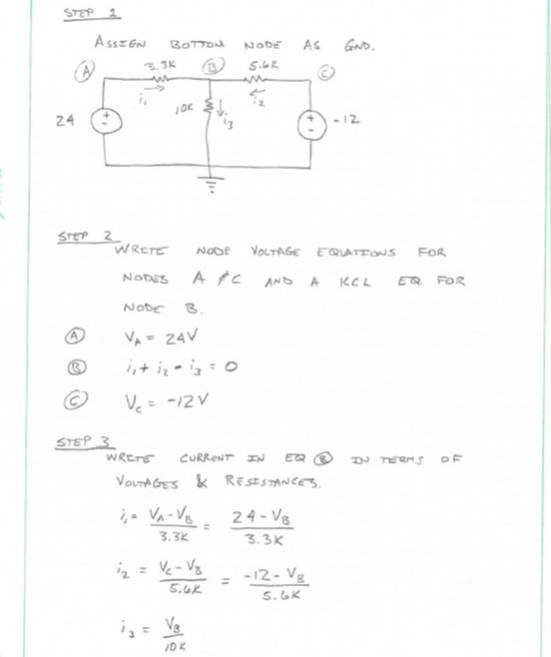
\includegraphics[width=0.55\textwidth]{TextbookExercise3-9solnM2-A.jpg}
\end{figure}
\begin{figure} [h t b]
\centering
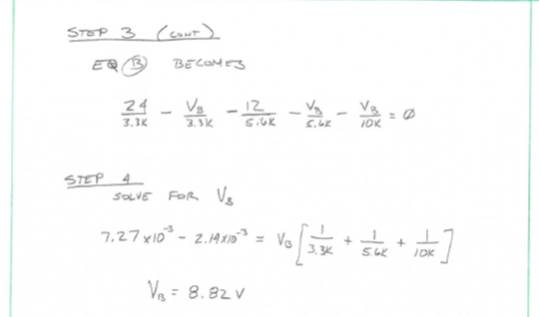
\includegraphics[width=0.5\textwidth]{TextbookExercise3-9solnM2-B.jpg}
\end{figure}
}

\newpage
\pagebreak
\clearpage
\subsection{Method 3: Use a SuperNode}
Method 3 is similar to method 2, except you to not have the reference node tied to your voltage sources.  A {\em Supernode} is just a combniation of the two nodes of a voltage source.  The supernode equation is
\begin{equation}
v_s = v_a-v_b
\end{equation}
where $v_s$ is the source voltage and $v_A$ \& $v_B$ are the node voltages on each side of teh source.

\textbf{Example}: Use any combination of the three methods above to solve for $I_0$ in the circuit shown in Figure \ref{fig: NodalAnalysisEx3}

\begin{figure} [h b t]
\centering
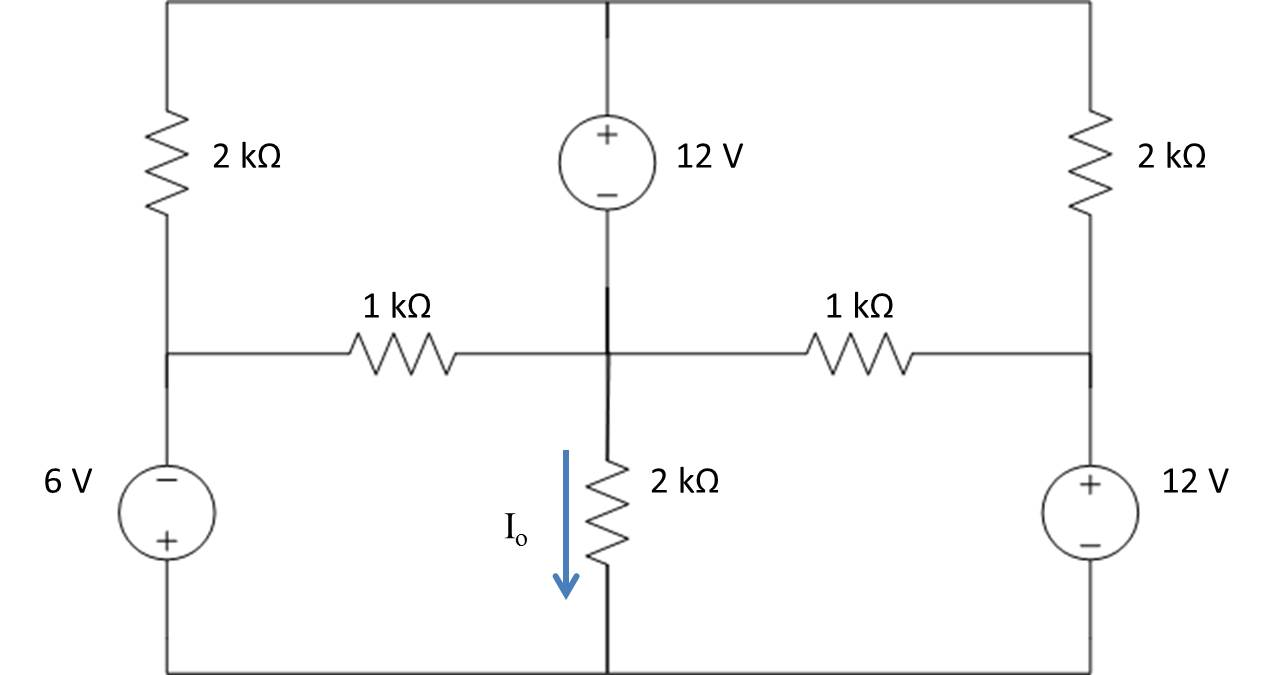
\includegraphics[width=0.6\textwidth]{NodalAnalysisEx3.jpg}
\caption{Circuit for Nodal Analysis Example}
\label{fig: NodalAnalysisEx3}
\end{figure}

\soln{7in}{
\begin{figure} [h t b]
\centering
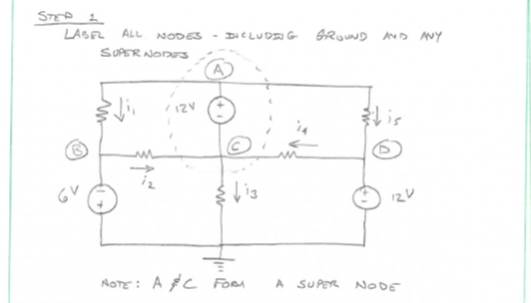
\includegraphics[width=0.75\textwidth]{NodalAnalysisEx3solnA.jpg}
\end{figure}
\begin{figure} [h t b]
\centering
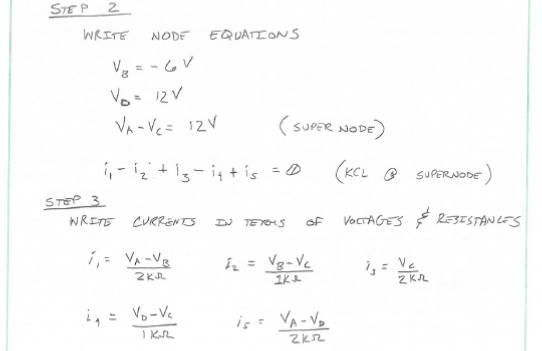
\includegraphics[width=0.6\textwidth]{NodalAnalysisEx3solnB.jpg}
\end{figure}
\begin{figure} [h t b]
\centering
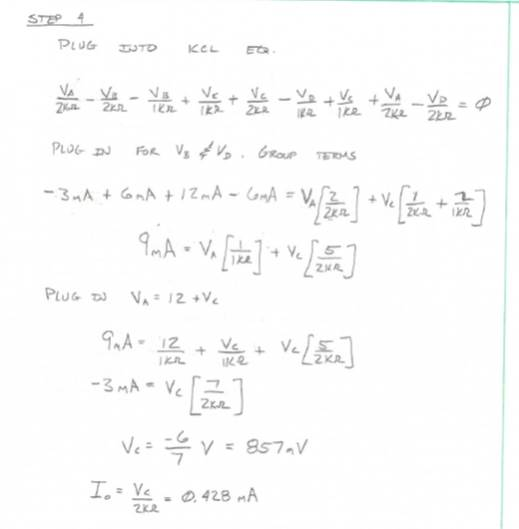
\includegraphics[width=0.6\textwidth]{NodalAnalysisEx3solnC.jpg}
\end{figure}
}

\newpage
\pagebreak
\clearpage

\section{Numerical Tools}

You can quickly solve these by use Matlab. Going back to Exercise 3-4, we can do:

% \soln{0.5in}{
	\begin{lstlisting}[language=Matlab,frame=single]
		A = [1.667, -0.667; -0.667 1.667]*1e-3
		b = [20; 50]*1e-3
		x = inv(A)*b
	\end{lstlisting}
% }

You can also use the Python programming language:

\begin{lstlisting}[language=Python,frame=single]
	import numpy as np
	A = np.array([[1.667, -0.667],[-0.667 1.667]]])*1e-3
	b = np.array([20, 50])*1e-3
	x = inv(A).dot(b)  # or x = np.linalg.solve(A,b)
\end{lstlisting}

Both are able to do numeric and symbolic manipulation.

%\section{Review Questions}
%\begin{questions}
%\item ......
%
%\soln{1in}{......}
%
%\newpage


%\end{questions}

\end{document}


% Equation Array Example Code
%\begin
%{eqnarray}
%P_R &=& i_R^2R \nonumber \\
%P_R &=& (100\ mA)^2 \times 100\ \Omega \nonumber \\
%P_R &=& (100 \times 10^{-3}\ A)^2 \times 100\ \Omega \\
%P_R &=& 10000 \times 10^{-6}\ A^2  \times 100\ \Omega \nonumber \\
%P_R &=& 1\ W  \nonumber
%\end{eqnarray}

% Figure Example Code
%\begin{figure}
%\centering
%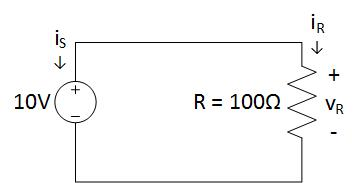
\includegraphics[width=0.5\textwidth]{OhmsLawExampleSolution.jpg}
%\caption{Ohm's Law example circuit}
%\label{fig: OhmsLawExampleSolution}
%\end{figure}

%Table Example Code
%\begin{table}[h]
%\centering
%\begin{tabular}{|l|c|c|}
%\hline
%Prefix & Abbreviation & Value \\
%\hline \hline
%Giga & $G$ & $10^9$ \\
%Mega & $M$ & $10^6$ \\
%Kilo & $k$ & $10^3$ \\
%\hline
%milli & $m$ & $10^{-3}$ \\
%micro & $\mu$ & $10^{-6}$ \\
%nano & $n$ & $10^{-9}$ \\
%pico & $p$ & $10^{-12}$ \\
%\hline
%\end{tabular}
%\caption{Engineering prefixes and values}
%\label{tab: Eng Prefixes}
%\end{table}
